\documentclass[11pt]{article}

\usepackage[a4paper,margin=1in]{geometry}
\usepackage[T1]{fontenc}
\usepackage[utf8]{inputenc}
\usepackage{lmodern}
\usepackage{microtype}
\usepackage{amsmath,amssymb,mathtools,bm}
\usepackage{booktabs}
\usepackage{array}
\usepackage{enumitem}
\usepackage{xcolor}
\usepackage{listings}
\usepackage{tikz}
\usetikzlibrary{arrows.meta,positioning,fit,calc}
\usepackage{hyperref}
\usepackage[nameinlink,noabbrev]{cleveref}

\hypersetup{
  colorlinks=true,
  linkcolor=blue!55!black,
  citecolor=blue!55!black,
  urlcolor=blue!55!black,
  pdftitle={An Even More Annotated Transformer},
  pdfauthor={Typeset from the supplied manuscript}
}

\definecolor{codebg}{RGB}{247,247,247}
\definecolor{codeframe}{RGB}{210,210,210}
\definecolor{codered}{RGB}{150,20,55}
\definecolor{codeblue}{RGB}{25,80,145}
\definecolor{codegreen}{RGB}{20,110,70}

\lstdefinestyle{pythonstyle}{
  language=Python,
  basicstyle=\ttfamily\footnotesize,
  keywordstyle=\color{codeblue}\bfseries,
  stringstyle=\color{codegreen},
  commentstyle=\color{black!55}\itshape,
  identifierstyle=\color{black},
  backgroundcolor=\color{codebg},
  frame=single,
  rulecolor=\color{codeframe},
  numbers=left,
  numberstyle=\tiny\color{black!45},
  numbersep=8pt,
  showstringspaces=false,
  breaklines=true,
  breakatwhitespace=false,
  columns=fullflexible,
  keepspaces=true,
  tabsize=4,
  captionpos=b
}
\lstset{style=pythonstyle}

\tikzset{
  block/.style={draw, rounded corners=2pt, thick, minimum width=3.2cm,
                minimum height=0.9cm, align=center, fill=blue!6},
  attn/.style={block, fill=orange!16, draw=orange!70!black},
  norm/.style={block, fill=green!11, draw=green!55!black},
  mlp/.style={block, fill=blue!10, draw=blue!60!black},
  embed/.style={block, fill=red!8, draw=red!55!black},
  output/.style={block, fill=purple!10, draw=purple!55!black},
  arrow/.style={-{Latex[length=2.5mm,width=1.6mm]}, thick},
  skip/.style={-{Latex[length=2.5mm,width=1.6mm]}, thick, dashed}
}

\title{An Even More Annotated Transformer\\
\large Architecture, Design Choices, Implementation, and Inference}
\author{Typeset and edited from the supplied manuscript}
\date{13 July 2023}

\newcommand{\R}{\mathbb{R}}
\newcommand{\softmax}{\operatorname{softmax}}
\newcommand{\LN}{\operatorname{LayerNorm}}
\newcommand{\MHA}{\operatorname{MHA}}
\newcommand{\FFN}{\operatorname{FFN}}
\newcommand{\Drop}{\operatorname{Dropout}}

\begin{document}
\maketitle

\begin{abstract}
This paper develops an implementation-oriented account of the Transformer architecture. It begins with scaled dot-product attention, interprets attention as a differentiable key--value lookup, and then derives multi-head attention. It proceeds through pre-layer-normalized encoder and decoder blocks, token and positional embeddings, weight tying, complete encoder--decoder assembly, teacher-forced training, and autoregressive inference. A compact PyTorch implementation is presented together with two experiments: sequence reversal and German--English machine translation. The final section discusses batching examples by length to reduce padding overhead.
\end{abstract}

\tableofcontents
\newpage

\section{Introduction}

The Transformer replaces sequential recurrent computation with attention-based interactions that can be evaluated in parallel across positions. The original architecture was introduced by Vaswani et al.~\cite{vaswani2017attention}; the presentation here follows the implementation-oriented tradition of the \emph{Annotated Transformer}~\cite{rush2018annotated}, while adding explicit discussion of dimensionality, variance, residual pathways, masking, normalization placement, and practical data handling.

Let an input sequence contain $T$ elements,
\[
X = \begin{bmatrix}x_1^\top & x_2^\top & \cdots & x_T^\top\end{bmatrix}^\top
\in \R^{T\times d_{\mathrm{model}}}.
\]
The central goal is to map each $x_i$ to a contextual representation $z_i$ that depends on the other sequence elements while avoiding the strictly sequential unrolling required by a recurrent neural network.

\section{Attention}
\label{sec:attention}

\subsection{Contextualizing independent encodings}

A simple linear encoding $W x_i$ can be evaluated independently for every position, but it does not couple position $i$ to the rest of the sequence. Self-attention introduces such coupling by computing a value vector for every element and then taking a data-dependent weighted average:
\begin{align}
  v_j &= x_j W_V, \\
  z_i &= \sum_{j=1}^{T} \alpha_{ij} v_j,
  \qquad \sum_{j=1}^{T}\alpha_{ij}=1,
  \qquad \alpha_{ij}\ge 0.
\end{align}
The weight $\alpha_{ij}$ should be large when element $i$ considers element $j$ relevant.

\subsection{Queries, keys, and values}

A symmetric score such as $x_i^\top x_j$ cannot distinguish ``$i$ attends to $j$'' from ``$j$ attends to $i$.'' The Transformer therefore learns separate query and key projections:
\begin{align}
  q_i &= x_i W_Q \in \R^{d_k}, \\
  k_j &= x_j W_K \in \R^{d_k}, \\
  v_j &= x_j W_V \in \R^{d_v}.
\end{align}
The unnormalized compatibility score is
\begin{equation}
  s_{ij}=\frac{q_i k_j^\top}{\sqrt{d_k}},
\end{equation}
and the attention weights are obtained row-wise by softmax:
\begin{equation}
  \alpha_{ij}
  =\frac{\exp(s_{ij})}{\sum_{m=1}^{T}\exp(s_{im})}.
\end{equation}
In matrix form,
\begin{equation}
\label{eq:scaled_attention}
  \operatorname{Attention}(Q,K,V)
  =\softmax\!\left(\frac{QK^\top}{\sqrt{d_k}}\right)V.
\end{equation}

\begin{figure}[htbp]
\centering
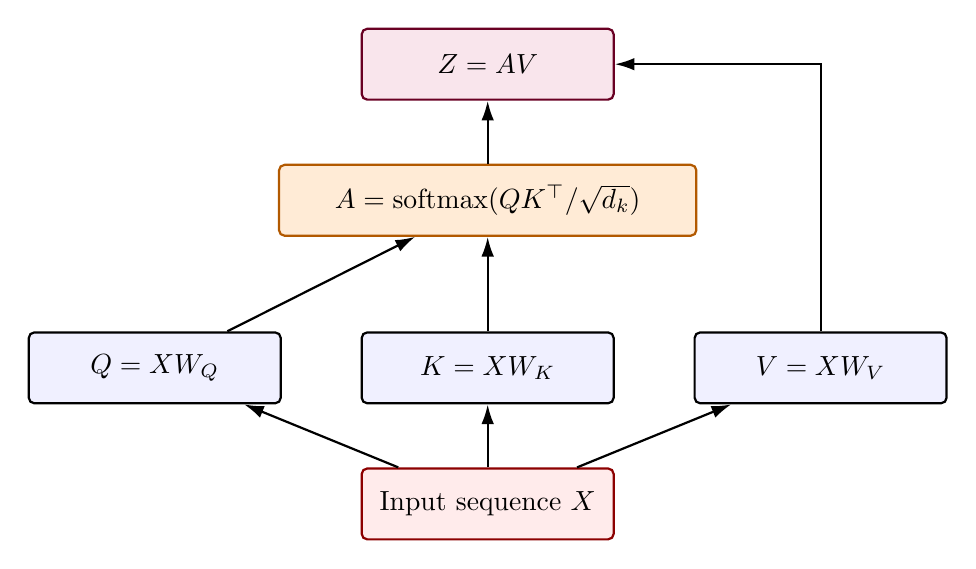
\begin{tikzpicture}[node distance=0.8cm and 1.0cm]
  \node[embed] (x) {Input sequence $X$};
  \node[block, above left=of x] (q) {$Q=XW_Q$};
  \node[block, above=of x] (k) {$K=XW_K$};
  \node[block, above right=of x] (v) {$V=XW_V$};
  \node[attn, above=1.2cm of k, minimum width=5.3cm] (score)
    {$A=\softmax(QK^\top/\sqrt{d_k})$};
  \node[output, above=of score] (z) {$Z=AV$};
  \draw[arrow] (x) -- (q);
  \draw[arrow] (x) -- (k);
  \draw[arrow] (x) -- (v);
  \draw[arrow] (q) -- (score);
  \draw[arrow] (k) -- (score);
  \draw[arrow] (score) -- (z);
  \draw[arrow] (v) |- (z);
\end{tikzpicture}
\caption{Scaled dot-product self-attention. All three projections are constructed from the same sequence in self-attention.}
\label{fig:self_attention}
\end{figure}

\subsection{Attention as a soft key--value lookup}

Equation~\eqref{eq:scaled_attention} can be interpreted as a differentiable lookup table. A conventional database matches a query to one discrete key and returns its associated value. Attention matches a query softly against every key, producing weights between zero and one, and returns the corresponding weighted combination of values. In self-attention, the key--value store is constructed from the same sequence being queried. In cross-attention, the keys and values come from an encoded source sequence, whereas the queries come from the target sequence.

\subsection{Why divide by $\sqrt{d_k}$?}

Assume that the components of $q$ and $k$ are independent, zero mean, and unit variance. Then
\begin{equation}
  qk^\top=\sum_{r=1}^{d_k}q_rk_r,
  \qquad
  \operatorname{Var}(qk^\top)=d_k.
\end{equation}
Thus the standard deviation of the raw dot product grows like $\sqrt{d_k}$. Large-magnitude logits make softmax nearly one-hot and produce small gradients for most entries. Dividing by $\sqrt{d_k}$ approximately restores unit-scale logits under this idealized initialization model.

\subsection{Masking}

Attention masks serve two common purposes:
\begin{enumerate}[label=(\alph*)]
  \item \textbf{Padding masks} remove padded sequence positions from the key--value store.
  \item \textbf{Causal masks} prevent target position $i$ from attending to future positions $j>i$.
\end{enumerate}
Operationally, forbidden logits are replaced by a large negative value before softmax:
\begin{equation}
  S_{ij}\leftarrow -\infty
  \quad\text{whenever position $j$ is masked for query $i$.}
\end{equation}
After softmax, the corresponding probability is zero.

\section{Multi-Head Attention}
\label{sec:mha}

A single attention distribution may concentrate on one dominant relation. Multi-head attention supplies $H$ independent query, key, and value projections so that different heads can represent distinct relations or subspaces:
\begin{align}
  \operatorname{head}_h
  &=\operatorname{Attention}
  \bigl(XW_Q^{(h)},XW_K^{(h)},XW_V^{(h)}\bigr), \\
  \MHA(X)
  &=\operatorname{Concat}
  \bigl(\operatorname{head}_1,\ldots,\operatorname{head}_H\bigr)W_O.
\end{align}
Typically $d_k=d_v=d_{\mathrm{model}}/H$, so concatenating all heads restores dimension $d_{\mathrm{model}}$ and avoids multiplying the leading parameter count by $H$.

Factoring the score through $W_Q$ and $W_K$ is also useful beyond the query--key metaphor. If the score were written directly as $x_i M x_j^\top$, then $M$ would be a full $d_{\mathrm{model}}\times d_{\mathrm{model}}$ matrix. Writing $M=W_QW_K^\top$ with $W_Q,W_K\in\R^{d_{\mathrm{model}}\times d_k}$ constrains $\operatorname{rank}(M)\le d_k$ and permits a lower-dimensional matching space.

\begin{lstlisting}[caption={Multi-head attention layer.},label={lst:mha_init}]
class MultiHeadAttention(nn.Module):
    def __init__(self, in_dim, qk_dim, v_dim, out_dim,
                 n_heads, attn_dropout=0.0):
        super().__init__()
        self.n_heads = n_heads
        self.Q = nn.Linear(in_dim, qk_dim, bias=False)
        self.K = nn.Linear(in_dim, qk_dim, bias=False)
        self.V = nn.Linear(in_dim, v_dim, bias=False)
        self.Wo = nn.Linear(v_dim, out_dim)
        self.attn_dropout = nn.Dropout(attn_dropout)

        head_qk = qk_dim // n_heads
        nn.init.normal_(
            self.Q.weight,
            std=np.sqrt(2.0 / (in_dim + head_qk)),
        )
        nn.init.normal_(
            self.K.weight,
            std=np.sqrt(2.0 / (in_dim + head_qk)),
        )
        nn.init.zeros_(self.Wo.bias)
\end{lstlisting}

The forward pass projects the three inputs, reshapes them into heads, computes scaled attention scores, applies an optional mask and dropout, concatenates the per-head outputs, and applies the output projection.

\begin{lstlisting}[caption={Forward pass of the multi-head attention layer.},label={lst:mha_forward}]
class MultiHeadAttention(nn.Module):
    # __init__ as above

    def forward(self, queries, keys, values, mask=None):
        B, T, _ = queries.shape
        _, Ts, _ = keys.shape

        if mask is not None:
            mask = mask.unsqueeze(dim=1)  # account for head dim

        q = self.Q(queries).view(B, T, self.n_heads, -1)
        q = q.transpose(1, 2)
        k = self.K(keys).view(B, Ts, self.n_heads, -1)
        k = k.transpose(1, 2)
        v = self.V(values).view(B, Ts, self.n_heads, -1)
        v = v.transpose(1, 2)

        scores = torch.matmul(q, k.transpose(2, 3))
        scores = scores / np.sqrt(k.shape[-1])

        if mask is not None:
            scores.masked_fill_(~mask, -1e9)

        attn = torch.softmax(scores, dim=-1)
        attn = self.attn_dropout(attn)

        z = torch.matmul(attn, v)
        z = z.transpose(1, 2).reshape(B, T, -1)
        out = self.Wo(z)
        return out, attn
\end{lstlisting}

Self-attention is invoked as
\begin{lstlisting}
z, attn = attn_layer(x, x, x)
\end{lstlisting}
whereas cross-attention passes a different sequence for keys and values.

Dropout is often applied directly to the attention probabilities during training. The retained entries no longer sum exactly to one in a particular dropout realization, but the operation is disabled during evaluation and its expectation is controlled by standard inverted dropout scaling.

\section{Encoder Block}
\label{sec:encoder}

An encoder consists of $N_{\mathrm{enc}}$ repeated blocks. Each block contains self-attention and a position-wise feed-forward network. The implementation considered here uses \emph{Pre-LayerNorm}:
\begin{align}
  U &= X + \Drop\bigl(\MHA(\LN(X))\bigr), \\
  Y &= U + \Drop\bigl(\FFN(\LN(U))\bigr),
\end{align}
with
\begin{equation}
  \FFN(x)=W_2\,\sigma(W_1x+b_1)+b_2.
\end{equation}
The inner dimension is usually several times $d_{\mathrm{model}}$; the original Transformer used $4d_{\mathrm{model}}$.

Residual connections make it possible for deeper stacks to approximate shallower ones by learning small residual updates. They also preserve a direct pathway for the initial token-plus-position representation. The feed-forward network contributes an element-wise nonlinear transformation; attention alone mainly forms data-dependent linear combinations of value vectors.

\begin{figure}[htbp]
\centering
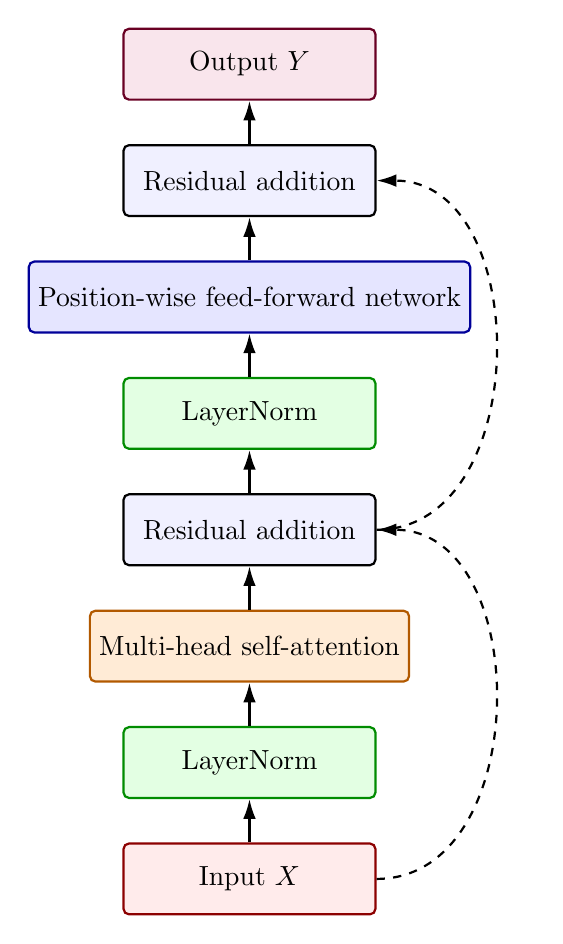
\begin{tikzpicture}[node distance=0.55cm]
  \node[embed] (x) {Input $X$};
  \node[norm, above=of x] (n1) {LayerNorm};
  \node[attn, above=of n1] (a) {Multi-head self-attention};
  \node[block, above=of a] (add1) {Residual addition};
  \node[norm, above=of add1] (n2) {LayerNorm};
  \node[mlp, above=of n2] (f) {Position-wise feed-forward network};
  \node[block, above=of f] (add2) {Residual addition};
  \node[output, above=of add2] (y) {Output $Y$};
  \foreach \u/\v in {x/n1,n1/a,a/add1,add1/n2,n2/f,f/add2,add2/y}
    \draw[arrow] (\u)--(\v);
  \draw[skip] (x.east) .. controls +(2.0,0) and +(2.0,0) .. (add1.east);
  \draw[skip] (add1.east) .. controls +(2.0,0) and +(2.0,0) .. (add2.east);
\end{tikzpicture}
\caption{Pre-LayerNorm encoder block. A final LayerNorm is applied after the complete encoder stack.}
\label{fig:encoder_block}
\end{figure}

\begin{lstlisting}[caption={Pre-LayerNorm encoder block.},label={lst:encoder}]
class EncoderBlock(nn.Module):
    def __init__(self, d_model, n_heads, dim_mlp, dropout):
        super().__init__()
        self.attn = MultiHeadAttention(
            in_dim=d_model,
            qk_dim=d_model,
            v_dim=d_model,
            out_dim=d_model,
            n_heads=n_heads,
            attn_dropout=dropout,
        )
        self.attn_dropout = nn.Dropout(dropout)
        self.attn_norm = nn.LayerNorm(d_model)

        self.mlp = nn.Sequential(
            nn.Linear(d_model, dim_mlp),
            nn.ReLU(),
            nn.Linear(dim_mlp, d_model),
        )
        self.mlp_dropout = nn.Dropout(dropout)
        self.mlp_norm = nn.LayerNorm(d_model)

    def forward(self, x, mask=None):
        attn_input = self.attn_norm(x)
        z, _ = self.attn(attn_input, attn_input,
                         attn_input, mask=mask)
        z = x + self.attn_dropout(z)

        r = self.mlp(self.mlp_norm(z))
        r = z + self.mlp_dropout(r)
        return r
\end{lstlisting}

The original Transformer used post-normalization, placing LayerNorm after each residual addition. Pre-LayerNorm places it before each sublayer and often improves optimization stability in deep models~\cite{xiong2020layernorm}. Because the residual stream is not normalized after each block, a final LayerNorm is added after the stack.

\section{Decoder Block}
\label{sec:decoder}

The decoder adds two mechanisms to the encoder pattern:
\begin{enumerate}
  \item masked self-attention over the target prefix;
  \item cross-attention from the target representation to encoder memory.
\end{enumerate}
For encoder memory $M$, a Pre-LayerNorm decoder block can be written as
\begin{align}
  U &= X + \Drop\bigl(\MHA_{\mathrm{causal}}(\LN(X))\bigr), \\
  C &= U + \Drop\bigl(\operatorname{CrossAttn}(\LN(U),M,M)\bigr), \\
  Y &= C + \Drop\bigl(\FFN(\LN(C))\bigr).
\end{align}
In cross-attention, queries come from the target stream, whereas keys and values come from the encoder output. For target length $T_{\mathrm{tgt}}$ and source length $T_{\mathrm{src}}$, each head produces an attention-score matrix of shape $T_{\mathrm{tgt}}\times T_{\mathrm{src}}$.

\begin{figure}[htbp]
\centering
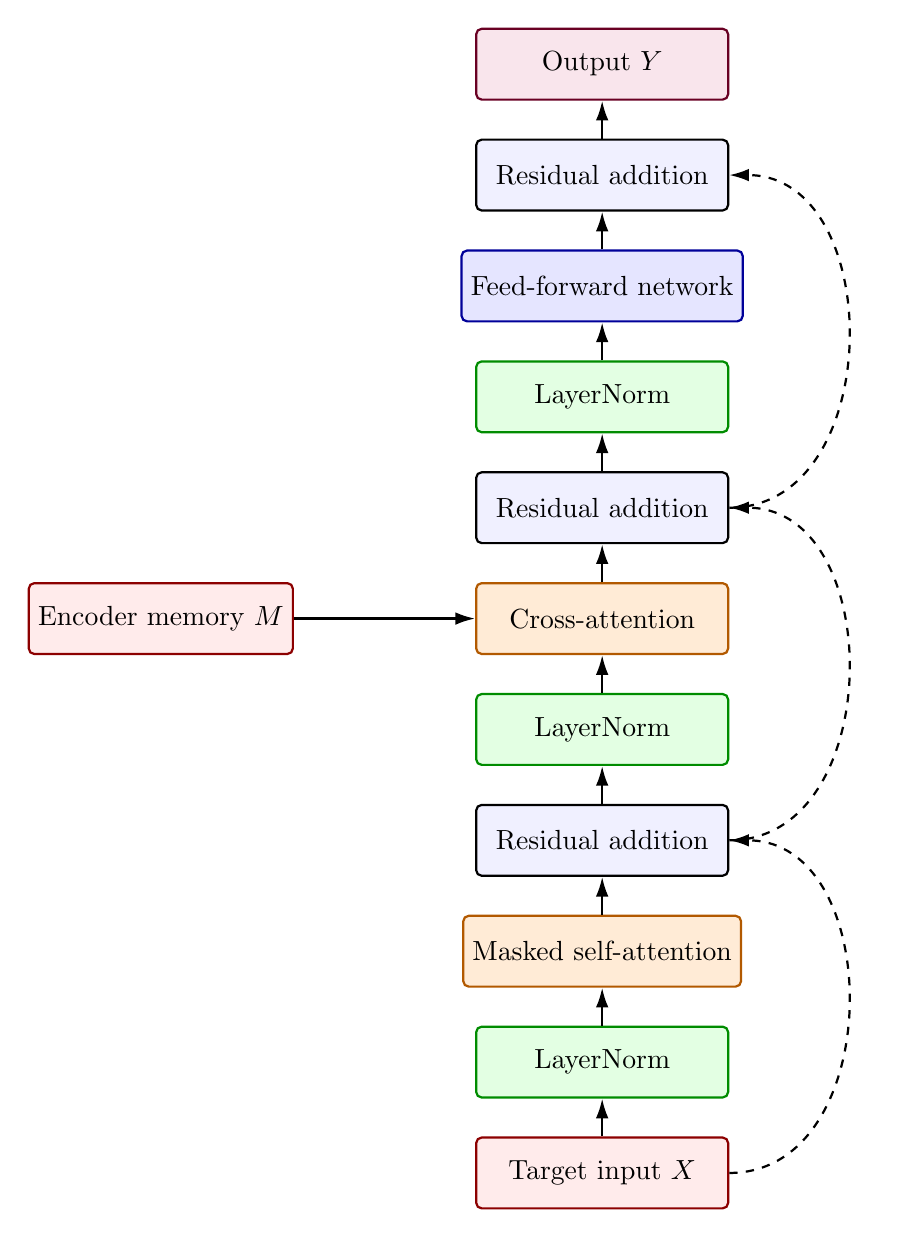
\begin{tikzpicture}[node distance=0.48cm]
  \node[embed] (x) {Target input $X$};
  \node[norm, above=of x] (n1) {LayerNorm};
  \node[attn, above=of n1] (sa) {Masked self-attention};
  \node[block, above=of sa] (a1) {Residual addition};
  \node[norm, above=of a1] (n2) {LayerNorm};
  \node[attn, above=of n2] (ca) {Cross-attention};
  \node[block, above=of ca] (a2) {Residual addition};
  \node[norm, above=of a2] (n3) {LayerNorm};
  \node[mlp, above=of n3] (ff) {Feed-forward network};
  \node[block, above=of ff] (a3) {Residual addition};
  \node[output, above=of a3] (y) {Output $Y$};
  \node[embed, left=2.3cm of ca] (mem) {Encoder memory $M$};
  \foreach \u/\v in {x/n1,n1/sa,sa/a1,a1/n2,n2/ca,ca/a2,a2/n3,n3/ff,ff/a3,a3/y}
    \draw[arrow] (\u)--(\v);
  \draw[arrow] (mem)--(ca);
  \draw[skip] (x.east) .. controls +(2.0,0) and +(2.0,0) .. (a1.east);
  \draw[skip] (a1.east) .. controls +(2.0,0) and +(2.0,0) .. (a2.east);
  \draw[skip] (a2.east) .. controls +(2.0,0) and +(2.0,0) .. (a3.east);
\end{tikzpicture}
\caption{Pre-LayerNorm decoder block with masked self-attention and encoder--decoder cross-attention.}
\label{fig:decoder_block}
\end{figure}

\begin{lstlisting}[caption={Pre-LayerNorm decoder block.},label={lst:decoder}]
class DecoderBlock(nn.Module):
    def __init__(self, d_model, n_heads, dim_mlp, dropout):
        super().__init__()
        self.self_attn = MultiHeadAttention(
            in_dim=d_model, qk_dim=d_model,
            v_dim=d_model, out_dim=d_model,
            n_heads=n_heads, attn_dropout=dropout,
        )
        self.self_attn_dropout = nn.Dropout(dropout)
        self.self_attn_norm = nn.LayerNorm(d_model)

        self.cross_attn = MultiHeadAttention(
            in_dim=d_model, qk_dim=d_model,
            v_dim=d_model, out_dim=d_model,
            n_heads=n_heads, attn_dropout=dropout,
        )
        self.cross_attn_dropout = nn.Dropout(dropout)
        self.cross_attn_norm = nn.LayerNorm(d_model)

        self.mlp = nn.Sequential(
            nn.Linear(d_model, dim_mlp),
            nn.ReLU(),
            nn.Linear(dim_mlp, d_model),
        )
        self.mlp_dropout = nn.Dropout(dropout)
        self.mlp_norm = nn.LayerNorm(d_model)

    def forward(self, x, mem, mem_mask=None):
        _, T, _ = x.shape
        causal_mask = torch.ones(
            1, T, T, dtype=torch.bool, device=x.device
        ).tril()

        qkv = self.self_attn_norm(x)
        z, _ = self.self_attn(qkv, qkv, qkv,
                              mask=causal_mask)
        z = x + self.self_attn_dropout(z)

        cross_query = self.cross_attn_norm(z)
        if mem_mask is not None:
            mem_mask = mem_mask.unsqueeze(dim=-2)
        c, _ = self.cross_attn(
            cross_query, mem, mem, mask=mem_mask
        )
        c = z + self.cross_attn_dropout(c)

        r = self.mlp(self.mlp_norm(c))
        r = c + self.mlp_dropout(r)
        return r
\end{lstlisting}

\section{Token and Position Embeddings}
\label{sec:embedding}

Encoder and decoder blocks accept vector sequences, not discrete token IDs. For vocabulary size $V$ and maximum sequence length $L_{\max}$, define a word embedding matrix $E_w\in\R^{V\times d_{\mathrm{model}}}$ and a positional embedding matrix $E_p\in\R^{L_{\max}\times d_{\mathrm{model}}}$. The representation at position $t$ is
\begin{equation}
\label{eq:embedding}
  e_t = s\,E_w[x_t] + E_p[t],
\end{equation}
where the original Transformer used $s=\sqrt{d_{\mathrm{model}}}$ and sinusoidal positions~\cite{vaswani2017attention}. The implementation below uses learned positional embeddings.

Self-attention is permutation equivariant: permuting the input rows permutes the output rows in the same way. Position information is therefore essential for language sequences.

\begin{lstlisting}[caption={Token-plus-position embedding layer.},label={lst:embedding}]
class TokenEmbedding(nn.Module):
    def __init__(self, word_embed_weight, pos_embed_weight,
                 scale, dropout):
        super().__init__()
        max_len, _ = pos_embed_weight.shape
        self.max_len = max_len
        self.word_embed_weight = word_embed_weight
        self.pos_embed_weight = pos_embed_weight
        self.dropout = nn.Dropout(dropout)

        positions = torch.arange(max_len).unsqueeze(dim=0)
        self.register_buffer("positions", positions)
        self.register_buffer(
            "scale", torch.tensor(float(scale))
        )

    def forward(self, x):
        _, T = x.shape
        if T > self.max_len:
            raise RuntimeError(
                "Sequence length exceeds maximum allowed limit"
            )

        pos = self.positions[:, :T]
        word_embed = F.embedding(x, self.word_embed_weight)
        pos_embed = F.embedding(pos, self.pos_embed_weight)
        embed = pos_embed + word_embed * self.scale
        return self.dropout(embed)
\end{lstlisting}

The source and target embedding matrices may be shared when vocabularies are compatible. The target embedding matrix can also be reused as the decoder output projection, a technique known as weight tying~\cite{press2017using}. Weight tying reduces parameters and often improves language-model performance, but initialization and scaling must keep the output logits in a numerically useful range.

\section{Complete Transformer}
\label{sec:transformer}

The complete encoder--decoder model consists of source and target embeddings, an encoder stack, a decoder stack, final normalizations, and a projection from decoder hidden states to target-vocabulary logits.

\begin{figure}[htbp]
\centering
\resizebox{0.93\textwidth}{!}{%
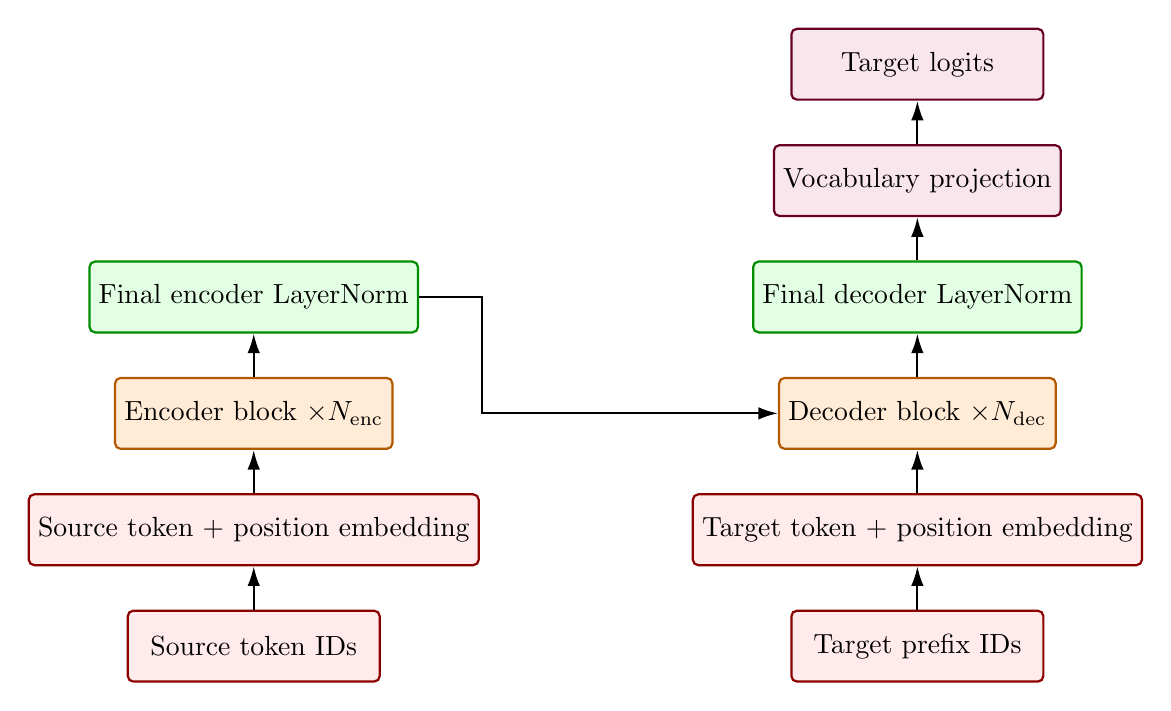
\begin{tikzpicture}[node distance=0.55cm and 2.2cm]
  \node[embed] (src) {Source token IDs};
  \node[embed, above=of src] (se) {Source token $+$ position embedding};
  \node[attn, above=of se] (enc) {Encoder block $\times N_{\mathrm{enc}}$};
  \node[norm, above=of enc] (en) {Final encoder LayerNorm};

  \node[embed, right=5.2cm of src] (tgt) {Target prefix IDs};
  \node[embed, above=of tgt] (te) {Target token $+$ position embedding};
  \node[attn, above=of te] (dec) {Decoder block $\times N_{\mathrm{dec}}$};
  \node[norm, above=of dec] (dn) {Final decoder LayerNorm};
  \node[output, above=of dn] (proj) {Vocabulary projection};
  \node[output, above=of proj] (logit) {Target logits};

  \draw[arrow] (src)--(se);
  \draw[arrow] (se)--(enc);
  \draw[arrow] (enc)--(en);
  \draw[arrow] (tgt)--(te);
  \draw[arrow] (te)--(dec);
  \draw[arrow] (dec)--(dn);
  \draw[arrow] (dn)--(proj);
  \draw[arrow] (proj)--(logit);
  \draw[arrow] (en.east)--++(0.8,0)|-(dec.west);
\end{tikzpicture}%
}
\caption{Complete Pre-LayerNorm Transformer. Encoder output is supplied as key--value memory to every decoder block.}
\label{fig:transformer}
\end{figure}

\begin{lstlisting}[caption={Transformer initialization.},label={lst:transformer_init}]
class Transformer(nn.Module):
    def __init__(self, src_vocab_size, tgt_vocab_size,
                 max_seq_len, d_model, n_heads,
                 n_enc, n_dec, dim_mlp, dropout):
        super().__init__()
        scale = np.sqrt(d_model)

        pos_embed = nn.Parameter(
            torch.randn(max_seq_len, d_model)
        )
        src_word_embed = nn.Parameter(
            torch.randn(src_vocab_size, d_model) / scale
        )

        if tgt_vocab_size is None:
            tgt_word_embed = src_word_embed
        else:
            tgt_word_embed = nn.Parameter(
                torch.randn(tgt_vocab_size, d_model) / scale
            )

        self.src_embed = TokenEmbedding(
            src_word_embed, pos_embed, scale, dropout
        )
        self.tgt_embed = TokenEmbedding(
            tgt_word_embed, pos_embed, scale, dropout
        )
        self.tgt_proj_weight = tgt_word_embed

        self.encoder_stack = nn.ModuleList(
            EncoderBlock(d_model, n_heads, dim_mlp, dropout)
            for _ in range(n_enc)
        )
        self.enc_norm = nn.LayerNorm(d_model)

        self.decoder_stack = nn.ModuleList(
            DecoderBlock(d_model, n_heads, dim_mlp, dropout)
            for _ in range(n_dec)
        )
        self.dec_norm = nn.LayerNorm(d_model)
\end{lstlisting}

\begin{lstlisting}[caption={Encoding, decoding, and teacher-forced forward pass.},label={lst:transformer_forward}]
class Transformer(nn.Module):
    # __init__ as above

    def encode(self, src, src_mask=None):
        z = self.src_embed(src)
        for encoder in self.encoder_stack:
            z = encoder(z, src_mask)
        return self.enc_norm(z)

    def decode(self, tgt, mem, mem_mask=None):
        z = self.tgt_embed(tgt)
        for decoder in self.decoder_stack:
            z = decoder(z, mem, mem_mask)
        return self.dec_norm(z)

    def forward(self, src, tgt, src_mask=None):
        mem = self.encode(src, src_mask)
        out = self.decode(tgt, mem, src_mask)
        tgt_scores = F.linear(out, self.tgt_proj_weight)
        return tgt_scores
\end{lstlisting}

For a batch size $B$, source length $T_s$, target length $T_t$, and target vocabulary size $V_t$, the principal tensor shapes are
\begin{center}
\begin{tabular}{@{}ll@{}}
\toprule
Quantity & Shape \\
\midrule
Source IDs & $B\times T_s$ \\
Target input IDs & $B\times T_t$ \\
Encoder memory & $B\times T_s\times d_{\mathrm{model}}$ \\
Decoder states & $B\times T_t\times d_{\mathrm{model}}$ \\
Target logits & $B\times T_t\times V_t$ \\
\bottomrule
\end{tabular}
\end{center}

During training, the decoder receives the ground-truth target shifted right. If the target is
\[
  [\mathrm{BOS},y_1,y_2,\ldots,y_T,\mathrm{EOS}],
\]
then the input and output arrays are
\begin{align}
  \texttt{tgt\_in}  &= [\mathrm{BOS},y_1,\ldots,y_T],\\
  \texttt{tgt\_out} &= [y_1,\ldots,y_T,\mathrm{EOS}].
\end{align}
This is teacher forcing: all target positions can be trained in parallel, while the causal mask ensures that position $t$ cannot use later target tokens.

\section{Autoregressive Inference}
\label{sec:inference}

At inference time, the true target sequence is unavailable. The encoder memory is computed once, and the decoder is repeatedly called on the generated prefix. Greedy decoding selects the largest-logit token at each step:
\begin{equation}
  \hat y_{t+1}=\arg\max_{v} z_{t,v}.
\end{equation}
The selected token is appended to the prefix, and decoding continues until an end-of-sequence token is produced or a maximum length is reached.

\begin{figure}[htbp]
\centering
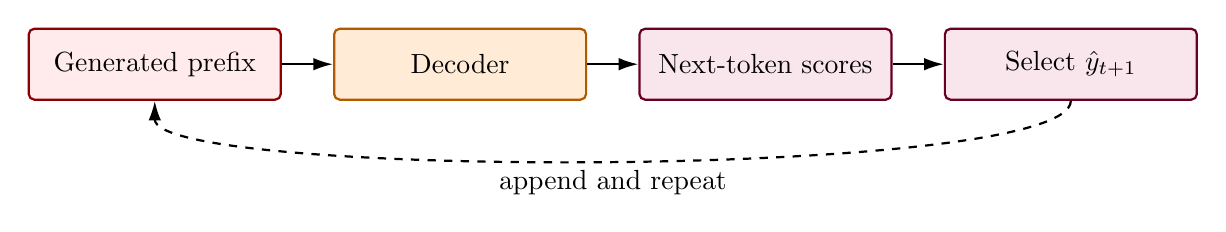
\begin{tikzpicture}[node distance=0.65cm and 0.65cm]
  \node[embed] (p) {Generated prefix};
  \node[attn, right=of p] (d) {Decoder};
  \node[output, right=of d] (s) {Next-token scores};
  \node[output, right=of s] (n) {Select $\hat y_{t+1}$};
  \draw[arrow] (p)--(d);
  \draw[arrow] (d)--(s);
  \draw[arrow] (s)--(n);
  \draw[skip] (n.south) .. controls +(0,-1.0) and +(0,-1.0) .. node[below]{append and repeat} (p.south);
\end{tikzpicture}
\caption{Autoregressive generation is an external loop around the non-recurrent Transformer decoder.}
\label{fig:inference}
\end{figure}

\begin{lstlisting}[caption={Greedy autoregressive decoding.},label={lst:greedy}]
class Transformer(nn.Module):
    # other methods as above

    @torch.no_grad()
    def greedy_decode(self, src, src_mask,
                      bos_idx, eos_idx, max_len=80):
        B = src.shape[0]
        done = torch.zeros(B, dtype=torch.bool,
                           device=src.device)
        was_training = self.training
        self.eval()

        tgt = torch.full(
            (B, 1), bos_idx,
            dtype=torch.long, device=src.device
        )
        mem = self.encode(src, src_mask)

        for _ in range(max_len - 1):
            out = self.decode(tgt, mem, mem_mask=src_mask)
            scores = F.linear(out, self.tgt_proj_weight)
            next_idx = scores[:, -1].argmax(dim=-1, keepdim=True)
            tgt = torch.cat((tgt, next_idx), dim=1)
            done |= next_idx.squeeze(-1).eq(eos_idx)
            if done.all():
                break

        if was_training:
            self.train()
        return tgt
\end{lstlisting}

Beginning- and end-of-sequence IDs are conventional control symbols rather than intrinsic requirements of the network. The model can be prompted with other vocabulary items, but termination behavior is most reliable when training explicitly associates a designated end token with sequence completion.

\section{Experiment I: Reversing a Sequence}
\label{sec:reverse}

A simple verification task is to reverse variable-length integer sequences. Each target is the reversed source surrounded by beginning- and end-of-sequence markers.

\begin{lstlisting}[caption={Synthetic reversal dataset.},label={lst:reverse_data}]
from random import randint
from torch.nn.utils.rnn import pad_sequence


device = torch.device(
    "cuda" if torch.cuda.is_available() else "cpu"
)
bos_idx, eos_idx, pad_idx = 1, 2, 0
vocab_size, src_len = 100, 16


def collate_reverse(batch):
    src = pad_sequence(
        batch, batch_first=True, padding_value=pad_idx
    )
    tgt = pad_sequence(
        [torch.tensor(
            [bos_idx] + x.flip(0).tolist() + [eos_idx]
        ) for x in batch],
        batch_first=True,
        padding_value=pad_idx,
    )
    return src, tgt


data_loader = data.DataLoader(
    dataset=[
        torch.randint(
            3, vocab_size,
            (randint(src_len // 2, src_len),)
        )
        for _ in range(50_000)
    ],
    batch_size=128,
    shuffle=True,
    drop_last=True,
    collate_fn=collate_reverse,
)
\end{lstlisting}

The model is deliberately small: two encoder blocks, two decoder blocks, $d_{\mathrm{model}}=64$, two heads, and an MLP width of 128. With a shared 100-token embedding table and 32 learned positions, this implementation has approximately $175{,}000$ trainable parameters.

\begin{lstlisting}[caption={Training and evaluating the reversal model.},label={lst:reverse_train}]
transformer = Transformer(
    src_vocab_size=vocab_size,
    tgt_vocab_size=None,
    max_seq_len=32,
    d_model=64,
    n_heads=2,
    n_enc=2,
    n_dec=2,
    dim_mlp=128,
    dropout=0.1,
).to(device)

optim = torch.optim.AdamW(
    transformer.parameters(),
    lr=1e-3,
    weight_decay=1e-4,
)

for _ in range(10):
    for src, tgt in data_loader:
        src, tgt = src.to(device), tgt.to(device)
        tgt_in, tgt_out = tgt[:, :-1], tgt[:, 1:]
        logits = transformer(src, tgt_in, src != pad_idx)
        loss = F.cross_entropy(
            logits.permute(0, 2, 1),
            tgt_out,
            ignore_index=pad_idx,
        )

        optim.zero_grad()
        loss.backward()
        torch.nn.utils.clip_grad_norm_(
            transformer.parameters(), 1.0
        )
        optim.step()

x = torch.tensor(
    [3, 5, 8, 13, 21, 34, 55, 89]
).unsqueeze(0).to(device)
y = transformer.greedy_decode(
    x, None, bos_idx, eos_idx, max_len=32
)
print(y)
# [1, 89, 55, 34, 21, 13, 8, 5, 3, 2]
\end{lstlisting}

The example highlights the shifted-target convention: the end token appears in the target output but not in the corresponding decoder input. Padding is excluded from the loss and from source attention through a Boolean mask.

\section{Experiment II: German--English Translation}
\label{sec:translation}

A more realistic test uses the Multi30K German--English dataset~\cite{elliott2016multi30k}. The following compact pipeline tokenizes both languages, constructs vocabularies with special symbols, and pads each batch.

\begin{lstlisting}[caption={Preparing Multi30K data.},label={lst:multi30k_data}]
from collections import Counter
from torch.nn.utils.rnn import pad_sequence
from torchtext.datasets import Multi30k
from torchtext.data.utils import get_tokenizer
from torchtext.vocab import vocab

train_data = Multi30k(root="datasets", split="train")
train_data = [
    (src, tgt) for src, tgt in train_data if len(src) > 0
]

UNK, PAD, BOS, EOS = (
    "<UNK>", "<PAD>", "<START>", "<END>"
)
tokenizer = get_tokenizer("basic_english")

de_counter, en_counter = Counter(), Counter()
for src, tgt in train_data:
    de_counter.update(tokenizer(src))
    en_counter.update(tokenizer(tgt))

de_vocab = vocab(
    de_counter, specials=[UNK, PAD, BOS, EOS]
)
en_vocab = vocab(
    en_counter, specials=[UNK, PAD, BOS, EOS]
)
de_vocab.set_default_index(de_vocab[UNK])
en_vocab.set_default_index(en_vocab[UNK])

pad_idx = de_vocab[PAD]
assert en_vocab[PAD] == pad_idx


def collate_translation(batch):
    src = pad_sequence(
        [torch.tensor(de_vocab(tokenizer(x)))
         for x, _ in batch],
        batch_first=True,
        padding_value=pad_idx,
    )
    tgt = pad_sequence(
        [torch.tensor(
            en_vocab([BOS] + tokenizer(y) + [EOS])
        ) for _, y in batch],
        batch_first=True,
        padding_value=pad_idx,
    )
    return src, tgt

train_loader = data.DataLoader(
    dataset=train_data,
    batch_size=128,
    shuffle=True,
    drop_last=True,
    collate_fn=collate_translation,
    num_workers=4,
)
\end{lstlisting}

\begin{lstlisting}[caption={Training the translation model.},label={lst:translation_train}]
transformer = Transformer(
    src_vocab_size=len(de_vocab),
    tgt_vocab_size=len(en_vocab),
    max_seq_len=256,
    d_model=256,
    n_heads=8,
    n_enc=4,
    n_dec=4,
    dim_mlp=512,
    dropout=0.1,
).to(device)

optim = torch.optim.AdamW(
    transformer.parameters(),
    lr=1e-4,
    weight_decay=1e-4,
)

for _ in range(30):
    for src, tgt in train_loader:
        src, tgt = src.to(device), tgt.to(device)
        tgt_in, tgt_out = tgt[:, :-1], tgt[:, 1:]
        src_mask = src != pad_idx

        logits = transformer(src, tgt_in, src_mask)
        loss = F.cross_entropy(
            logits.permute(0, 2, 1),
            tgt_out,
            ignore_index=pad_idx,
        )

        optim.zero_grad()
        loss.backward()
        torch.nn.utils.clip_grad_norm_(
            transformer.parameters(), 1.0
        )
        optim.step()
\end{lstlisting}

A representative source sentence and greedy translation are
\begin{lstlisting}[caption={Example translation.},label={lst:translation_example}]
sent = [
    "zwei", "frauen", "spazieren", "und",
    "lachen", "im", "park", "."
]
x = torch.tensor(de_vocab(sent)).unsqueeze(0).to(device)
y = transformer.greedy_decode(
    x, None, en_vocab[BOS], en_vocab[EOS]
)
print(en_vocab.lookup_tokens(y[0].tolist()))
# ['<START>', 'two', 'women', 'are', 'walking',
#  'and', 'laughing', 'in', 'the', 'park', '.', '<END>']
\end{lstlisting}

The example is intentionally modest and is not intended as a competitive translation benchmark. Its purpose is to verify that the same implementation supports a genuine source--target language task.

\section{Batching by Sequence Length}
\label{sec:batching}

Padding is computationally wasteful because attention operates on the padded rectangular batch. Grouping examples of similar lengths reduces this overhead. A practical compromise is to shuffle indices globally, divide them into moderately large pools, sort each pool by sequence length, and then form batches from adjacent sorted examples.

\begin{lstlisting}[caption={Length-aware batch sampler.},label={lst:batch_sampler}]
class BatchSampler:
    def __init__(self, lengths, batch_size):
        self.lengths = lengths
        self.batch_size = batch_size

    def __iter__(self):
        size = len(self.lengths)
        indices = list(range(size))
        random.shuffle(indices)

        step = 100 * self.batch_size
        for i in range(0, size, step):
            pool = indices[i:i + step]
            pool = sorted(
                pool, key=lambda idx: self.lengths[idx]
            )

            for j in range(0, len(pool), self.batch_size):
                if j + self.batch_size > len(pool):
                    break  # drop_last=True
                yield pool[j:j + self.batch_size]

    def __len__(self):
        return len(self.lengths) // self.batch_size
\end{lstlisting}

The sampler is supplied through the \texttt{batch\_sampler} argument rather than through the ordinary batch-size and shuffle arguments. In the reported experiment, the average number of padding tokens per sequence decreased from approximately $15.25$ to $3.62$.

\begin{lstlisting}[caption={Using the length-aware sampler.},label={lst:batch_loader}]
lengths = [len(src) for src, _ in train_data]
batch_size = 128

train_loader = data.DataLoader(
    dataset=train_data,
    batch_sampler=BatchSampler(lengths, batch_size),
    collate_fn=collate_translation,
    num_workers=4,
)

avg_pads = sum(
    (src == pad_idx).sum() / src.shape[0]
    for src, _ in train_loader
) / len(train_loader)
\end{lstlisting}

\section{Discussion}

Several design choices interact:
\begin{itemize}
  \item \textbf{Attention and parallelism.} Unlike recurrent unrolling, attention computes all query positions in parallel during training.
  \item \textbf{Multi-head factorization.} Splitting a fixed model width across heads creates multiple learned relation spaces without increasing the dominant projection dimension.
  \item \textbf{Residual pathways and normalization.} Residual additions preserve a direct information and gradient path. Pre-LayerNorm usually improves optimization stability, while final normalization restores controlled output scale.
  \item \textbf{Feed-forward sublayers.} The position-wise MLP adds nonlinearity and feature transformation after attention mixes information across positions. Other domains may substitute different local transformations; for example, FastSpeech uses convolutional sublayers in its feed-forward Transformer blocks~\cite{ren2019fastspeech}.
  \item \textbf{Weight tying.} Sharing target embeddings and output projection reduces parameters and can improve generalization, provided initialization and scaling remain appropriate.
  \item \textbf{Training versus generation.} Teacher forcing exposes the entire shifted target during training, whereas inference feeds previous model predictions back into an external autoregressive loop.
\end{itemize}

\section{Conclusion}

The Transformer can be understood as a composition of a few precise operations: learned token and position representations, scaled dot-product attention, head concatenation and output projection, position-wise nonlinear processing, residual connections, and normalization. The encoder turns a source sequence into contextual memory; the decoder combines causal target self-attention with queries into that memory. The accompanying implementation makes these abstractions explicit and demonstrates them on both a controlled reversal task and a small machine-translation example. Practical performance depends not only on architecture but also on masking, initialization, target shifting, gradient control, and efficient batching.

\begin{thebibliography}{9}

\bibitem{vaswani2017attention}
A. Vaswani, N. Shazeer, N. Parmar, J. Uszkoreit, L. Jones,
A. N. Gomez, L. Kaiser, and I. Polosukhin,
``Attention Is All You Need,''
\emph{Advances in Neural Information Processing Systems}, vol. 30, 2017.

\bibitem{rush2018annotated}
A. M. Rush,
``The Annotated Transformer,'' 2018.
\url{https://nlp.seas.harvard.edu/annotated-transformer/}

\bibitem{ren2019fastspeech}
Y. Ren, Y. Ruan, X. Tan, T. Qin, S. Zhao, Z. Zhao, and T.-Y. Liu,
``FastSpeech: Fast, Robust and Controllable Text to Speech,''
\emph{Advances in Neural Information Processing Systems}, vol. 32, 2019.

\bibitem{xiong2020layernorm}
R. Xiong, Y. Yang, D. He, K. Zheng, S. Zheng, C. Xing,
H. Zhang, Y. Lan, L. Wang, and T.-Y. Liu,
``On Layer Normalization in the Transformer Architecture,''
\emph{Proceedings of the 37th International Conference on Machine Learning}, 2020.

\bibitem{press2017using}
O. Press and L. Wolf,
``Using the Output Embedding to Improve Language Models,''
\emph{Proceedings of the 15th Conference of the European Chapter of the Association for Computational Linguistics}, 2017.

\bibitem{elliott2016multi30k}
D. Elliott, S. Frank, K. Sima'an, and L. Specia,
``Multi30K: Multilingual English--German Image Descriptions,''
\emph{Proceedings of the 5th Workshop on Vision and Language}, 2016.

\end{thebibliography}

\end{document}
